\section{Experimental Evaluation}
\label{sec:experimental-evaluation}

We evaluate two linked questions for log-based activity association: whether command and action traces can retrieve same-task trajectories across execution modes under difficult candidate sets, and whether an explicit execution-mode score improves that ranking. The evaluation establishes a concrete behavioral-retrieval baseline and shows that mode information changes association quality differently across query directions.

\subsection{Data and protocol}
\label{sec:data-protocol}

We use a pinned release of the public Cyber Task Horizons collection (commit \texttt{178c0da1800f9c07311e1b8d6c61dd8104e7b4ae}; \url{https://github.com/lyptus-research/cyber-task-horizons-data/tree/178c0da1800f9c07311e1b8d6c61dd8104e7b4ae}), combining InterCode-CTF, CyBench, and NYUCTF. The paired subset contains 177 non-empty traces from 40 benchmark--task groups: 57 expert terminal traces and 120 Agent tool-call traces. The Agent subset contains 40 traces each from Claude Sonnet 4.6, Claude Opus 4.6, and GPT-5.5. We use only observable command tokens and coarse action sequences; prompts, task descriptions, tool outputs, answers, model names, timestamps, and paths are excluded from the association features. Python tool calls are excluded from the primary representation.

All records for a \texttt{benchmark/task\_id} remain in one of five outer folds. For each held-out query, candidates come only from the same benchmark; the matching task ID is the positive and other task IDs are hard negatives. Vocabulary, TF--IDF weights, ProcGrep patterns, mode classifiers, and association rankers are fit on training tasks only. The mode-aware ranker uses inner-fold, out-of-fold mode scores for training pairs and outer-fold predictions for test pairs. We report benchmark-macro Recall@1, mean reciprocal rank (MRR), and query AUC. Confidence intervals use 5,000 task-cluster bootstrap replicates, stratified by benchmark; each benchmark contributes equally to the macro-average.

\subsection{Behavioral traces retrieve same-task Agent activity above random ranking}
\label{sec:cross-mode-retrieval}

The strongest simple representation is the ordered coarse-action bigram model, with Human-to-Agent Recall@1 of 0.414 (95\% task-cluster CI [0.245, 0.576]), MRR 0.561, and query AUC 0.733. It reaches the highest point estimate among the four representation baselines and matches the mode-aware prototype's Recall@1 point estimate. The other simple baselines obtain Recall@1 values of 0.347 for command unigrams, 0.265 for ordered command bigrams, and 0.287 for ProcGrep local patterns; their intervals and full metrics appear in Appendix~\ref{app:complete-results}. The benchmark-macro random-ranking baseline is 0.116.

The same ordering signal appears within each benchmark: ordered-action-bigram Recall@1 is 0.417 on CyBench (6 tasks; random 0.167), 0.111 on InterCode-CTF (27 tasks; random 0.037), and 0.714 on NYUCTF (7 tasks; random 0.143). The absolute values vary substantially across suites, so the pooled result is best read as evidence that command-level traces contain task-discriminative structure under same-benchmark negatives, with benchmark-specific difficulty determining its strength. Figure~\ref{fig:retrieval} reports the task-cluster intervals and complete representation comparison.

\begin{figure}[tb]
  \centering
  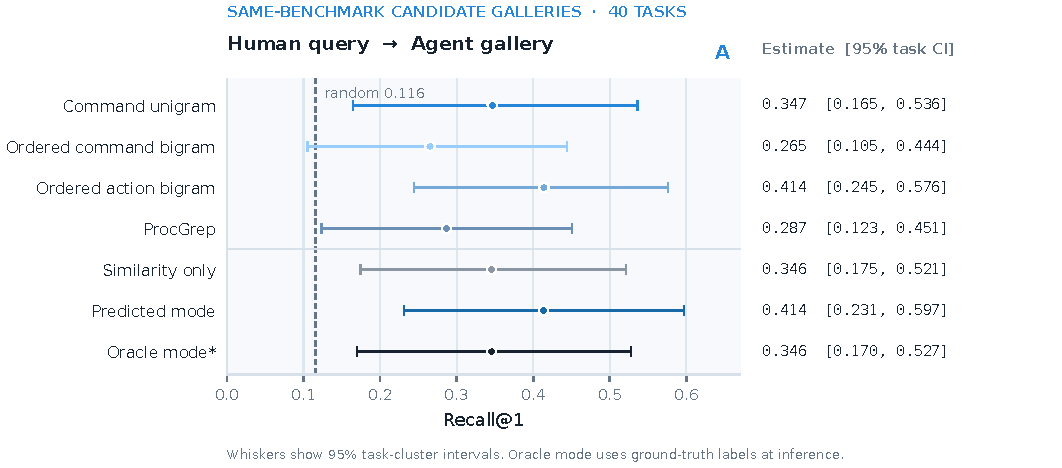
\includegraphics[width=\linewidth]{figure1_retrieval.pdf}
  \caption{Human-to-Agent same-task retrieval with same-benchmark hard negatives. Points show benchmark-macro Recall@1 and whiskers show 95\% task-cluster bootstrap intervals. The dashed line marks the macro random-ranking baseline (0.116). The oracle-mode row uses ground-truth mode labels at inference and is included only as a diagnostic. Task identity is a CTF challenge proxy, not an attack-activity label.}
  \label{fig:retrieval}
\end{figure}

\subsection{Execution-mode information has direction-dependent effects}
\label{sec:mode-effects}

Adding out-of-fold mode scores changes Human-to-Agent Recall@1 from 0.346 to 0.414, a paired gain of 0.068 across 40 task groups. The paired 95\% interval is [\(-0.012\), 0.191]; corresponding changes in MRR (0.039, CI [\(-0.006\), 0.100]) and query AUC (0.015, CI [\(-0.005\), 0.040]) also span zero. The estimate centers on a 6.8-point gain, but it does not resolve whether this direction benefits reliably. The oracle-mode diagnostic returns Recall@1 0.346, matching the similarity-only point estimate. Since every Human-to-Agent comparison already has the same ground-truth mode pair, the predicted-score gain cannot be attributed to the binary mode label alone; it may reflect within-class score structure or capture-process cues.

The paired analysis reveals the more consequential result: the effect depends on the query--candidate mode relation. Human-to-Human Recall@1 decreases by 0.098 (95\% CI [\(-0.189\), \(-0.007\)]; 17 eligible task groups), whereas Agent-to-Agent cross-model and Agent-to-Human changes are small and their intervals span zero. Thus, adding a global mode correction can trade performance across association directions rather than uniformly improve retrieval. Figure~\ref{fig:mode-effects} makes this asymmetry explicit. Our prototype consequently treats execution mode as an observable relation feature whose contribution must be assessed per query direction, with the mode score kept distinct from behavioral similarity.

\begin{figure}[tb]
  \centering
  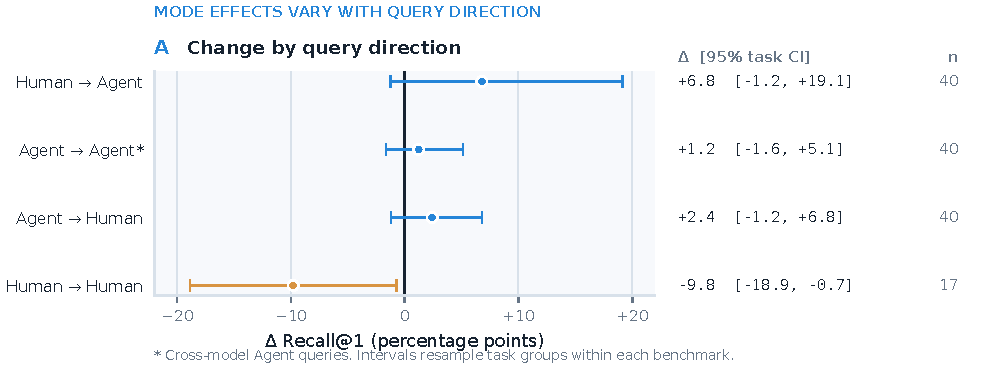
\includegraphics[width=\linewidth]{figure2_mode_effects.pdf}
  \caption{Paired change in Recall@1 after adding predicted execution-mode features to the similarity-only ranker. Positive values favor the mode-aware ranker. Intervals resample task groups within benchmark; \(n\) counts eligible independent task groups. Agent-to-Agent queries use different source models.}
  \label{fig:mode-effects}
\end{figure}

\subsection{Mode-label prediction measures trace separability, not actor identity}
\label{sec:mode-classification}

The command n-gram mode head obtains balanced accuracy 0.863 (95\% CI [0.804, 0.915]), macro-F1 0.854, and ROC AUC 0.945 (95\% CI [0.917, 0.972]) on the paired trace set. A command-count/action-mixture control reaches AUC 0.728, while benchmark identity alone reaches AUC 0.501. This pattern shows that execution-mode labels are predictable from the recorded traces beyond benchmark identity. It also shows why the classifier cannot yet be interpreted as an actor detector: expert activity is recorded as terminal input and Agent activity as tool calls, so label and capture pathway are aligned. The result motivates a same-sensor evaluation in which operator and execution mode vary independently.

\subsection{Resulting research claim}
\label{sec:resulting-claim}

Across the evaluated public traces, task-level behavioral retrieval is measurable under same-benchmark hard negatives, while predicted execution-mode information changes ranking quality in a direction-dependent way. This supports a focused association-layer design: expose execution mode as an explicit, query-conditioned signal and evaluate its contribution alongside behavioral similarity. The present evidence establishes the benchmark and prototype behavior needed to test that design; the activity-level experiment must use repeated executions with shared telemetry and independent activity identifiers.
